\section{Results}

The model performed better than using the average
recipe in predicting the U.S. \gls{UNF}, without
a large increase in computational time.


\subsection{Depletion Calculation Time and File Size}

For 100 random sets of
burnup and enrichment depletion calculations,
the model takes 0.12 seconds, while
searching the database for an assembly
with the closest burnup and enrichment (using Pandas read csv)
takes 21.8 seconds. Also, the pickled model file is only
38 Kb, while the curated database (.csv) is 330 Mb.

\subsection{Assembly Comparison}

Ten burnup and enrichment data was picked at random from the \gls{UDB},
and was compared with the model predictions, to observe
two things:
\begin{enumerate}
    \item What isotope (or Z, A range) the model is good / bad
        at predicting
    \item What burnup / enrichment range the model is good / bad
        at predicting
\end{enumerate}

Figures \ref{fig:28_33681}, \ref{fig:324_33536},
\ref{fig:349_40150}, and \ref{fig:401_47722}
show that the model
generally has a high relative error percentage for Ra-226
(average concentration 6.0 e-12\%) ,Ac-227 (average concentration  2.3 e-12\%), and curium isotopes.
The absolute prediction errors are quite small
(\textasciitilde 1e-11), but the percent errors are large due
to the small value of the data. There was not a notable
difference in the error values for enrichment
and burnup variations.

\begin{figure}
    \centering
    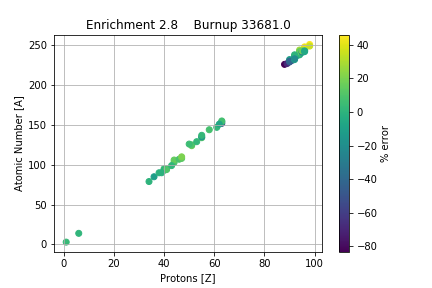
\includegraphics[width=\textwidth]{2-8_33681-0.png}
    \caption{Isotope by isotope prediction error percentage
             plotted for a discrete burnup and enrichment.}
    \label{fig:28_33681}
\end{figure}


\begin{figure}
    \centering
    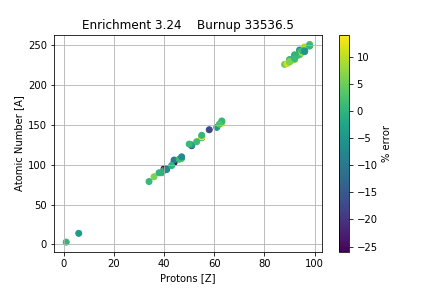
\includegraphics[width=\textwidth]{3-24_33536-5.png}
    \caption{Isotope by isotope prediction error percentage
             plotted for a discrete burnup and enrichment.
             }
    \label{fig:324_33536}
\end{figure}



\begin{figure}
    \centering
    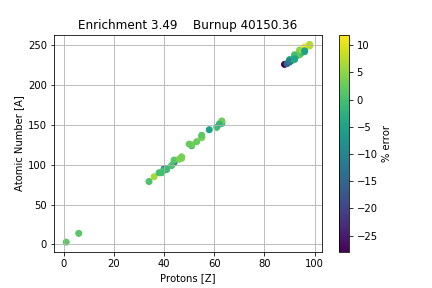
\includegraphics[width=\textwidth]{3-49_40150-36.png}
    \caption{Isotope by isotope prediction error percentage
             plotted for a discrete burnup and enrichment.
             }
    \label{fig:349_40150}
\end{figure}


\begin{figure}
    \centering
    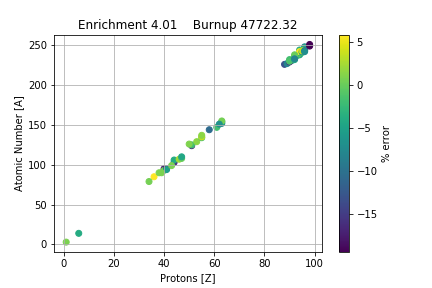
\includegraphics[width=\textwidth]{4-01_47722-32.png}
    \caption{Isotope by isotope prediction error percentage
             plotted for a discrete burnup and enrichment.
             }
    \label{fig:401_47722}
\end{figure}

A general plot of 


\subsection{U.S. \gls{UNF} Inventory Comparison}

In this section we compare three \gls{UNF} inventories.
The inventories are acquired by using the assembly mass data
in the \gls{UDB}. The only difference is the composition of the
assemblies. The three different inventories acquire the recipe by:
\begin{enumerate}
    \item Data: simply importing from database
    \item Prediction: model prediction of composition using burnup and enrichment from database
    \item Recipe: using average recipe (for all assemblies)
\end{enumerate}

We compare the three inventories on the three
metrics:
\begin{enumerate}
    \item Isotopic inventory
    \item Waste metrics (activity and decay heat)
    \item Equivalent fissile inventory (equivalent pu-239)
\end{enumerate}

The Unified database contains discharged assembly data
from nuclear reactors in the United States up to May of
2013. We added all the \gls{UNF} assemblies in the database.


\begin{table}[h]
    \centering
    \begin{tabular}{lrrr}
        \hline
        Metric & Data & Recipe & Prediction \\
        \hline
        $^{239}Pu$ mass [t] & 320.37 & 305.14 & 318.51\\
        $^{137}Cs$ mass [t] & 63.84 & 58.46 & 63.15 \\
        $^{235}U$ mass [t] & 464.60 & 455.18 & 454.31\\
        $^{238}U$ mass [t] & 42,171 & 42,200 & 42,213\\
        \hline
        Decay Heat [MW] & 193.39 & 208.25 & 191.77 \\
        Activity [Bq] & $2.79e21$ & $2.15e21$ & $2.74e21$ \\
        \hline
    \end{tabular}
    \caption{Comparison of \gls{PWR} \gls{UNF} inventory in the U.S.}
\end{table}

\FloatBarrier

\subsubsection{Isotope Inventory}

Comparing the isotope inventory, the model outperforms the
average recipe method for all isotopes.
Figure \ref{fig:iso_rel} shows the relative
error between the full database, model prediction, and
average recipe for
major isotopes. For plutonium isotopes, the model far
outperforms the average database.

\begin{figure}
    \centering
    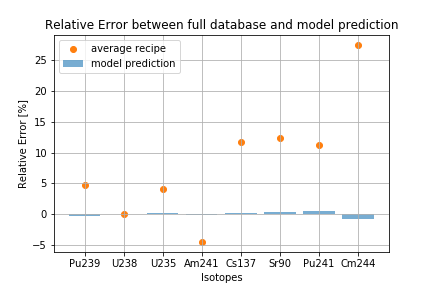
\includegraphics[width=\textwidth]{iso_rel.png}
    \caption{Relative error percentage of important isotopes}
    \label{fig:iso_rel}
\end{figure}


\begin{figure}
    \centering
    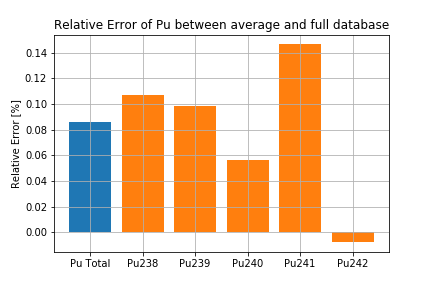
\includegraphics[width=\textwidth]{pu_rel.png}
    \caption{Relative error percentage for plutonium isotopes.}
    \label{fig:pu_rel}
\end{figure}

\FloatBarrier


\subsubsection{Waste Metric}
The model excellently predicts the waste metrics activity
and decay heat. Figures \ref{fig:assem_dh} and \ref{fig:assem_act}
show the relative error percent of the decay heat and activity
predictions per assembly. The model predicts most assemblies
with an error less than 1\%, except for assemblies with low
burnup.
Figures \ref{fig:assem_dh_recipe} and
\ref{fig:assem_act_recipe} show the relative error percent
of the decay heat and activity from the average recipe.
As shown the error is higher as the point is farther from
the average burnup and enrichment.


\begin{figure}
    \centering
    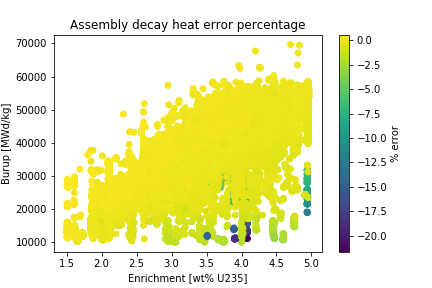
\includegraphics[width=\textwidth]{assem_dh.png}
    \caption{Relative error percentage for predicting the decay
             heat of individual assemblies.}
    \label{fig:assem_dh}
\end{figure}


\begin{figure}
    \centering
    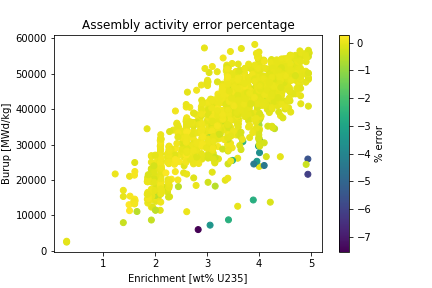
\includegraphics[width=\textwidth]{assem_act.png}
    \caption{Relative error percentage for predicting the
             activity of individual assemblies.}
    \label{fig:assem_act}
\end{figure}


\begin{figure}
    \centering
    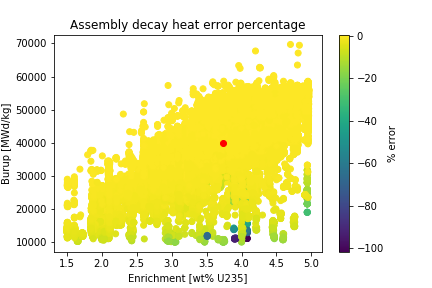
\includegraphics[width=\textwidth]{assem_dh_recipe.png}
    \caption{Relative error percentage for decay heat
             of the average recipe
             method. The red point is the average enrichment and
             burnup.}
    \label{fig:assem_dh_recipe}
\end{figure}

\begin{figure}
    \centering
    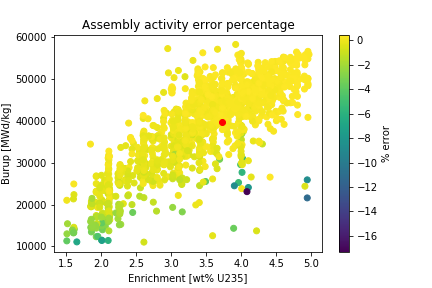
\includegraphics[width=\textwidth]{assem_act_recipe.png}
    \caption{Relative error percentage for activity
             of the assembly of the average recipe
             method. The red point is the average enrichment and
             burnup.}
    \label{fig:assem_act_recipe}
\end{figure}

\FloatBarrier


Table \ref{tab:wm} shows the decay heat and activity value
comparison in years 2020, 2100, and 3100. The total
error is less than 1.1\% for all metrics at all time periods.
Figure \ref{fig:ha_err} shows the relative error percentage
of activity and decay heat progression in time. It shows
that the model outperforms the average recipe method
in predicting waste metrics.


\begin{table}[h]
    \centering
    \begin{tabular}{lcrrr}
        \hline
        Metric & Year & Data & Prediction  & Error [\%] \\
        \hline
        \multirow{3}{*}{\shortstack{Decay \\ Heat}} & 2020 & 41.01 & 40.83 & 0.43 \\
                                                    & 2100 & 16.43 & 16.39 & 0.23 \\
                                                    & 3100 & 3.14 & 3.13 & 0.085 \\
        \hline
        \multirow{3}{*}{\shortstack{Activity}} & 2020 & 4.67e20 & 4.62e20 & 1.07 \\
                                               & 2100 & 6.39e19 & 6.32e19 & 1.09 \\
                                               & 3100 & 3.68e18 & 3.68e18 & 0.061 \\
        \hline
    \end{tabular}
    \caption{Decay heat and radioactivity values and errors for years 2020, 2100, and 3100.}
    \label{tab:wm}
\end{table}

\begin{figure}
    \centering
    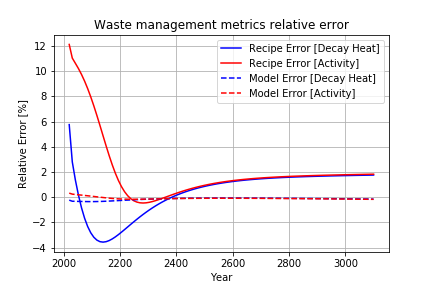
\includegraphics[width=\textwidth]{ha_err.png}
    \caption{Relative error of waste management metrics for \gls{UNF} inventory
             generated by the average recipe, and the prediction model.}
    \label{fig:ha_err}
\end{figure}

\FloatBarrier

\subsubsection{Assembly fissile quality}

Fissile quality is calculated as a metric called
equivalent plutonium-239, shown in figure \ref{fig:pu_equiv} \cite{anon_plutonium_1989}. This value is
calculated by aggregating the weighted fissile
values of each isotope in an \gls{UNF}.
For example, the equivalent fissile value for
an \gls{LWR} will be calculated by:
\begin{equation}
\text{Pu}_{eq} = 0.8(U_{235}) - (\text{Pu}_{238}) + (\text{Pu}_{239}) - 0.4(\text{Pu}_{240}) \\
            + 1.3(\text{Pu}_{241}) - 1.4(\text{Pu}_{242}) - 2.2(\text{Am}_{241})
\end{equation}
Where the isotopes represent the mass of each isotope.


\begin{figure}
    \centering
    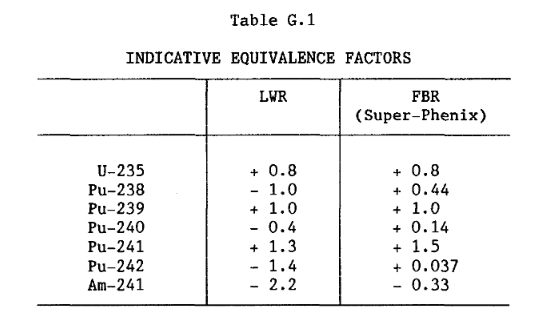
\includegraphics[width=\textwidth]{pu_equiv.png}
    \caption{Equivalent factors of each isotope for
             calculating equivalent Pu-239 value,
             from \cite{anon_plutonium_1989}. Factors
             are separated by reactor neutron spectrum
             due to cross section variations in different
             spectra.}
    \label{fig:pu_equiv}
\end{figure}

Figure \ref{fig:fiss} shows the fast equivalent Pu-239
value of the \gls{UNF} inventory plotted over time.
The trained model outperforms the recipe method. The
initial falls for all three lines are due to the
decay of plutonium 241, which has a half-life of
14 years.

\begin{figure}
    \centering
    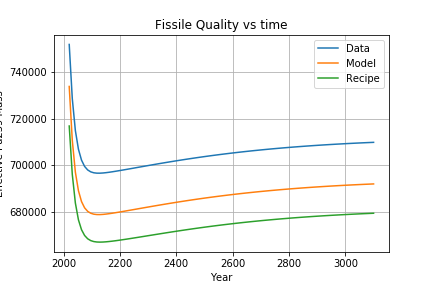
\includegraphics[width=\textwidth]{fiss.png}
    \caption{fast factors were used}
    \label{fig:fiss}
\end{figure}




\subsection{\Cyclus implementation}

Applications and use cases

We can simulate transition scenarios of different future
burnup of \gls{LWR} fuel increases over time and how that
affects transition time.

This model allows simulation of a dynamic \gls{PWR}, where
the burnup, enrichment, cycle time and refuel time can be
highly customizable. This capability allows a modeling of a
\gls{PWR} fleet with varying performances, while the performance
changes with time.

[one single reactor with varying assemblies received and sent]

\FloatBarrier